\documentclass{article}

\usepackage[utf8]{inputenc}
\usepackage{geometry}
\usepackage{graphicx}
\usepackage{titling}
\usepackage{fancyhdr}
\usepackage{cmbright}
\usepackage{caption}
\usepackage{subcaption}

\geometry{
	a4paper,
	total={170mm, 257mm},
	left=20mm,
	top=20mm
}


\title{Chapter 8: Space, Things and Movements}
\author{Fharook Shaik}
\date{05 January 2025}

\fancypagestyle{fancy}{
	\fancyhf{}
	\fancyfoot[R]{
\includegraphics[width=3cm]{images/BTULogo_englisch_grau_2x.png}}
	\fancyfoot[L]{\thedate}
	\fancyhead[L]{13869 - Braitenberg Vehicle Praktium}
	\fancyhead[R]{\theauthor}
}

\pagestyle{fancy}

\makeatletter
\renewcommand{\maketitle}{
	\thispagestyle{fancy}
	\null
	\vskip 1em
	\begin{center}
		{\LARGE \@title \par}
	\end{center}
	\vskip 3em
}
\makeatother


\begin{document}

	\maketitle

	\noindent\begin{tabular}{@{}ll}
		Student & \theauthor\\
		Professor &  Dr. Cunningham, Douglas\\
		Matrikel-Nr.: & 5014962
		 
	\end{tabular}

	\section*{Summary}

    In Chapter 8, the focus shifts to the introduction of internal spatial representations in vehicles. By equipping Vehicle 8 with organized arrays of sensors and networks for processing input, the chapter explores how these enhancements allow vehicles to perceive their environment more effectively. These internal maps not only simplify the vehicle's wiring but also enable it to detect objects, recognize motion, and navigate its surroundings with a deeper understanding of space.

	The chapter begins with the concept of a \textit{map} within the vehicle. Instead of scattering sensors randomly, the sensors are arranged in a neat grid, such as a 10x10 array of photocells. A lens fitted over this grid creates a camera-like system, projecting an image of the environment onto the array. While the resolution is limited, this setup provides a clear representation of the order and spatial relationships of objects in the vehicle's surroundings. This orderly mapping of sensory data becomes the foundation for Vehicle 8's ability to process and interpret spatial information.

	\begin{figure}[h]
		\centering
		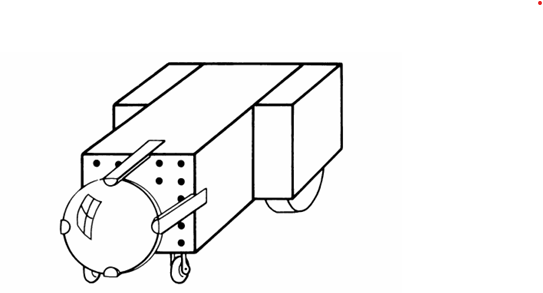
\includegraphics[scale=0.6]{images/figure_11.png}
		\caption{Vehicle 8 with a lense eye}
		\label{fig:vehicle-8}
	\end{figure}

	\subsection*{Detecting Objects and Recognizing Movements}
	Vehicle 8 uses networks of threshold devices to process input from its photocell array, enabling it to detect objects and recognize movements. Object detection occurs when groups of neighboring photocells activate the same threshold device. For instance, if a large object appears nearby, the threshold device connected to that region of the photocell array becomes strongly activated, allowing the vehicle to identify significant objects while ignoring smaller, less relevant details.

	The vehicle's ability to recognize movement builds on this principle. Each photocell connects to a delay device and a neighboring photocell through a threshold device. When a moving object passes from left to right, the first photocell activates the delay device, which holds the signal briefly. By the time the object activates the next photocell, both signals reach the threshold device simultaneously, activating it. This setup allows the vehicle to detect motion directionally, distinguishing left-to-right movement from right-to-left. By tuning the network, the vehicle can also track motion at specific speeds or recognize objects of particular sizes in motion.

	These capabilities can be combined for greater functionality. For example, object detectors can feed into movement detectors, enabling the vehicle to identify moving objects of specific sizes. Alternatively, movement detectors can inform object detectors, helping the vehicle recognize objects as collections of points moving in unison. This process mirrors human perception, such as recognizing camouflaged creatures by their motion against a background.

	\begin{figure}
		\centering
		\begin{minipage}{.5\textwidth}
		  \centering
		  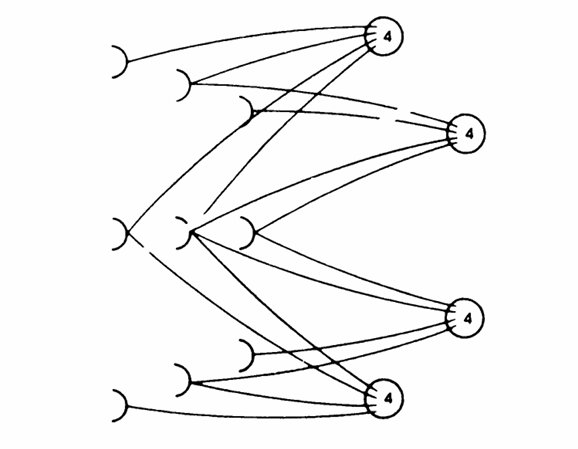
\includegraphics[width=.7\linewidth]{images/figure_12.png}
		  \captionof{figure}{An Object Detector each of threshold devices on the right responds only whenfour neighbouring sensors arranged in a square are active together}
		\end{minipage}%
		\qquad
		\begin{minipage}{.5\textwidth}
		  \centering
		  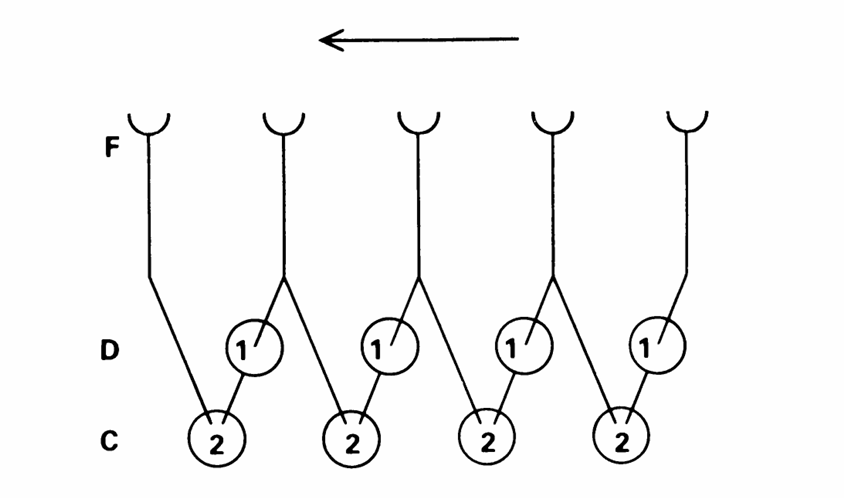
\includegraphics[width=.7\linewidth]{images/figure_13.png}
		  \captionof{figure}{Set of movement detectors (C) for movement from right to left. Threshold devices C will be active when they receive input directly from the sensor F and input from delay element D at the same time.}
		\end{minipage}
	\end{figure}

	\subsection*{Perception with Lateral Inhibiion}
	
	Another important feature introduced in this chapter is lateral inhibition, which sharpens the vehicle's sensory processing. In this system, each threshold device inhibits the activity of its neighbors, ensuring that only the strongest signals are processed. This technique highlights distinct features, such as isolated bright spots, while filtering out uniform or uninteresting stimuli. By focusing on high-contrast areas, the vehicle can better detect meaningful patterns in its environment.

	\subsection*{Internal Representations of Space}

	The chapter emphasizes the importance of internal spatial representations for processing sensory data. While the examples focus on two-dimensional visual space, the same principles apply to other sensory modalities. For instance, a three-dimensional tactile map could represent points touched by a jointed arm equipped with sensors. Similarly, stereoscopic vision could allow the vehicle to perceive depth in three-dimensional space.

	The concept extends beyond human comprehension, with networks capable of representing higher-dimensional spaces, such as four dimensions. By connecting discrete points in a network with lines representing neighborhood relationships, the vehicle can navigate spaces that humans cannot visualize. For example, a four-dimensional network allows the vehicle to process complex spatial relationships and \textit{navigate} higher-dimensional spaces.

	The chapter proposes ways to test whether Vehicle 8 truly understands space. For example, if the vehicle is moved away from a favorable location and seeks to return, its ability to take the shortest diagonal path instead of retracing its steps suggests an understanding of two-dimensional Euclidean geometry. Such behavior demonstrates the vehicle's ability to use an internal map to navigate efficiently.

	Additionally, the vehicle's networks can analyze physical reality by evaluating motion continuity and object consistency. For instance, the vehicle can determine whether an image's motion aligns with physical laws, ensuring it represents a real object. Similarly, networks can detect changes in a shadow's shape or maintain object recognition despite movement, further enhancing the vehicle's understanding of its environment.

	\begin{figure}
		\centering
		\begin{minipage}{.6\textwidth}
		  \centering
		  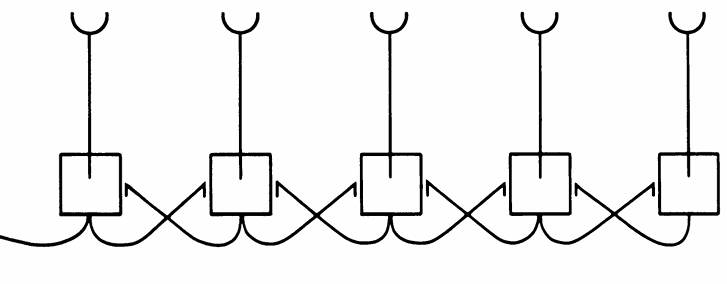
\includegraphics[width=.7\linewidth]{images/figure_14.png}
		  \captionof{figure}{Five threshold devices, excited by many sensors, each connected o its neighbours by inhibitory connections}
		\end{minipage}%
		\qquad
		\begin{minipage}{.6\textwidth}
		  \centering
		  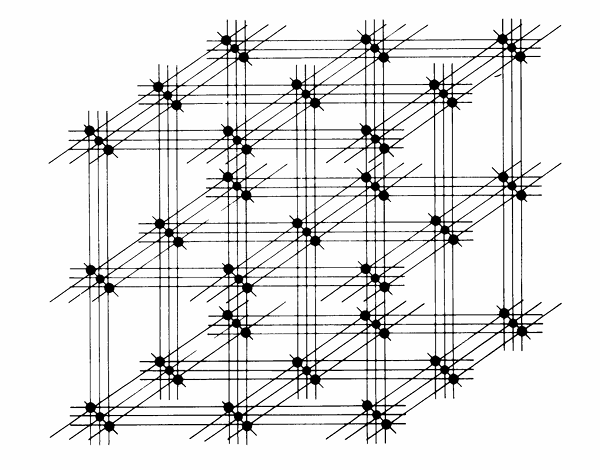
\includegraphics[width=.7\linewidth]{images/figure_15.png}
		  \captionof{figure}{A four dimensional cube. Each edge marked by three black dos on a line, connected by a wire.}
		\end{minipage}
	\end{figure}

	\subsection*{Conclusion}

	Chapter 8 illustrates how internal spatial representations transform Vehicle 8's ability to perceive and interact with its environment. By organizing sensory inputs and processing them through networks of threshold devices, the vehicle can detect objects, recognize motion, and navigate complex spaces. These internal maps provide a framework for interpreting the world, enabling the vehicle to respond with precision and adaptability.

	This chapter highlights the connection between spatial dimensionality and perception, showing how orderly representations of space—whether two-dimensional, three-dimensional, or beyond—equip vehicles with powerful tools for navigating and understanding their surroundings. Through these advancements, Vehicle 8 demonstrates the profound potential of internal maps in creating systems capable of intelligent behavior.

\end{document}